\documentclass[twoside]{report}

\usepackage{project}

\backgroundsetup{
scale=1,
color=black,
opacity=1,
angle=0,
contents={%
  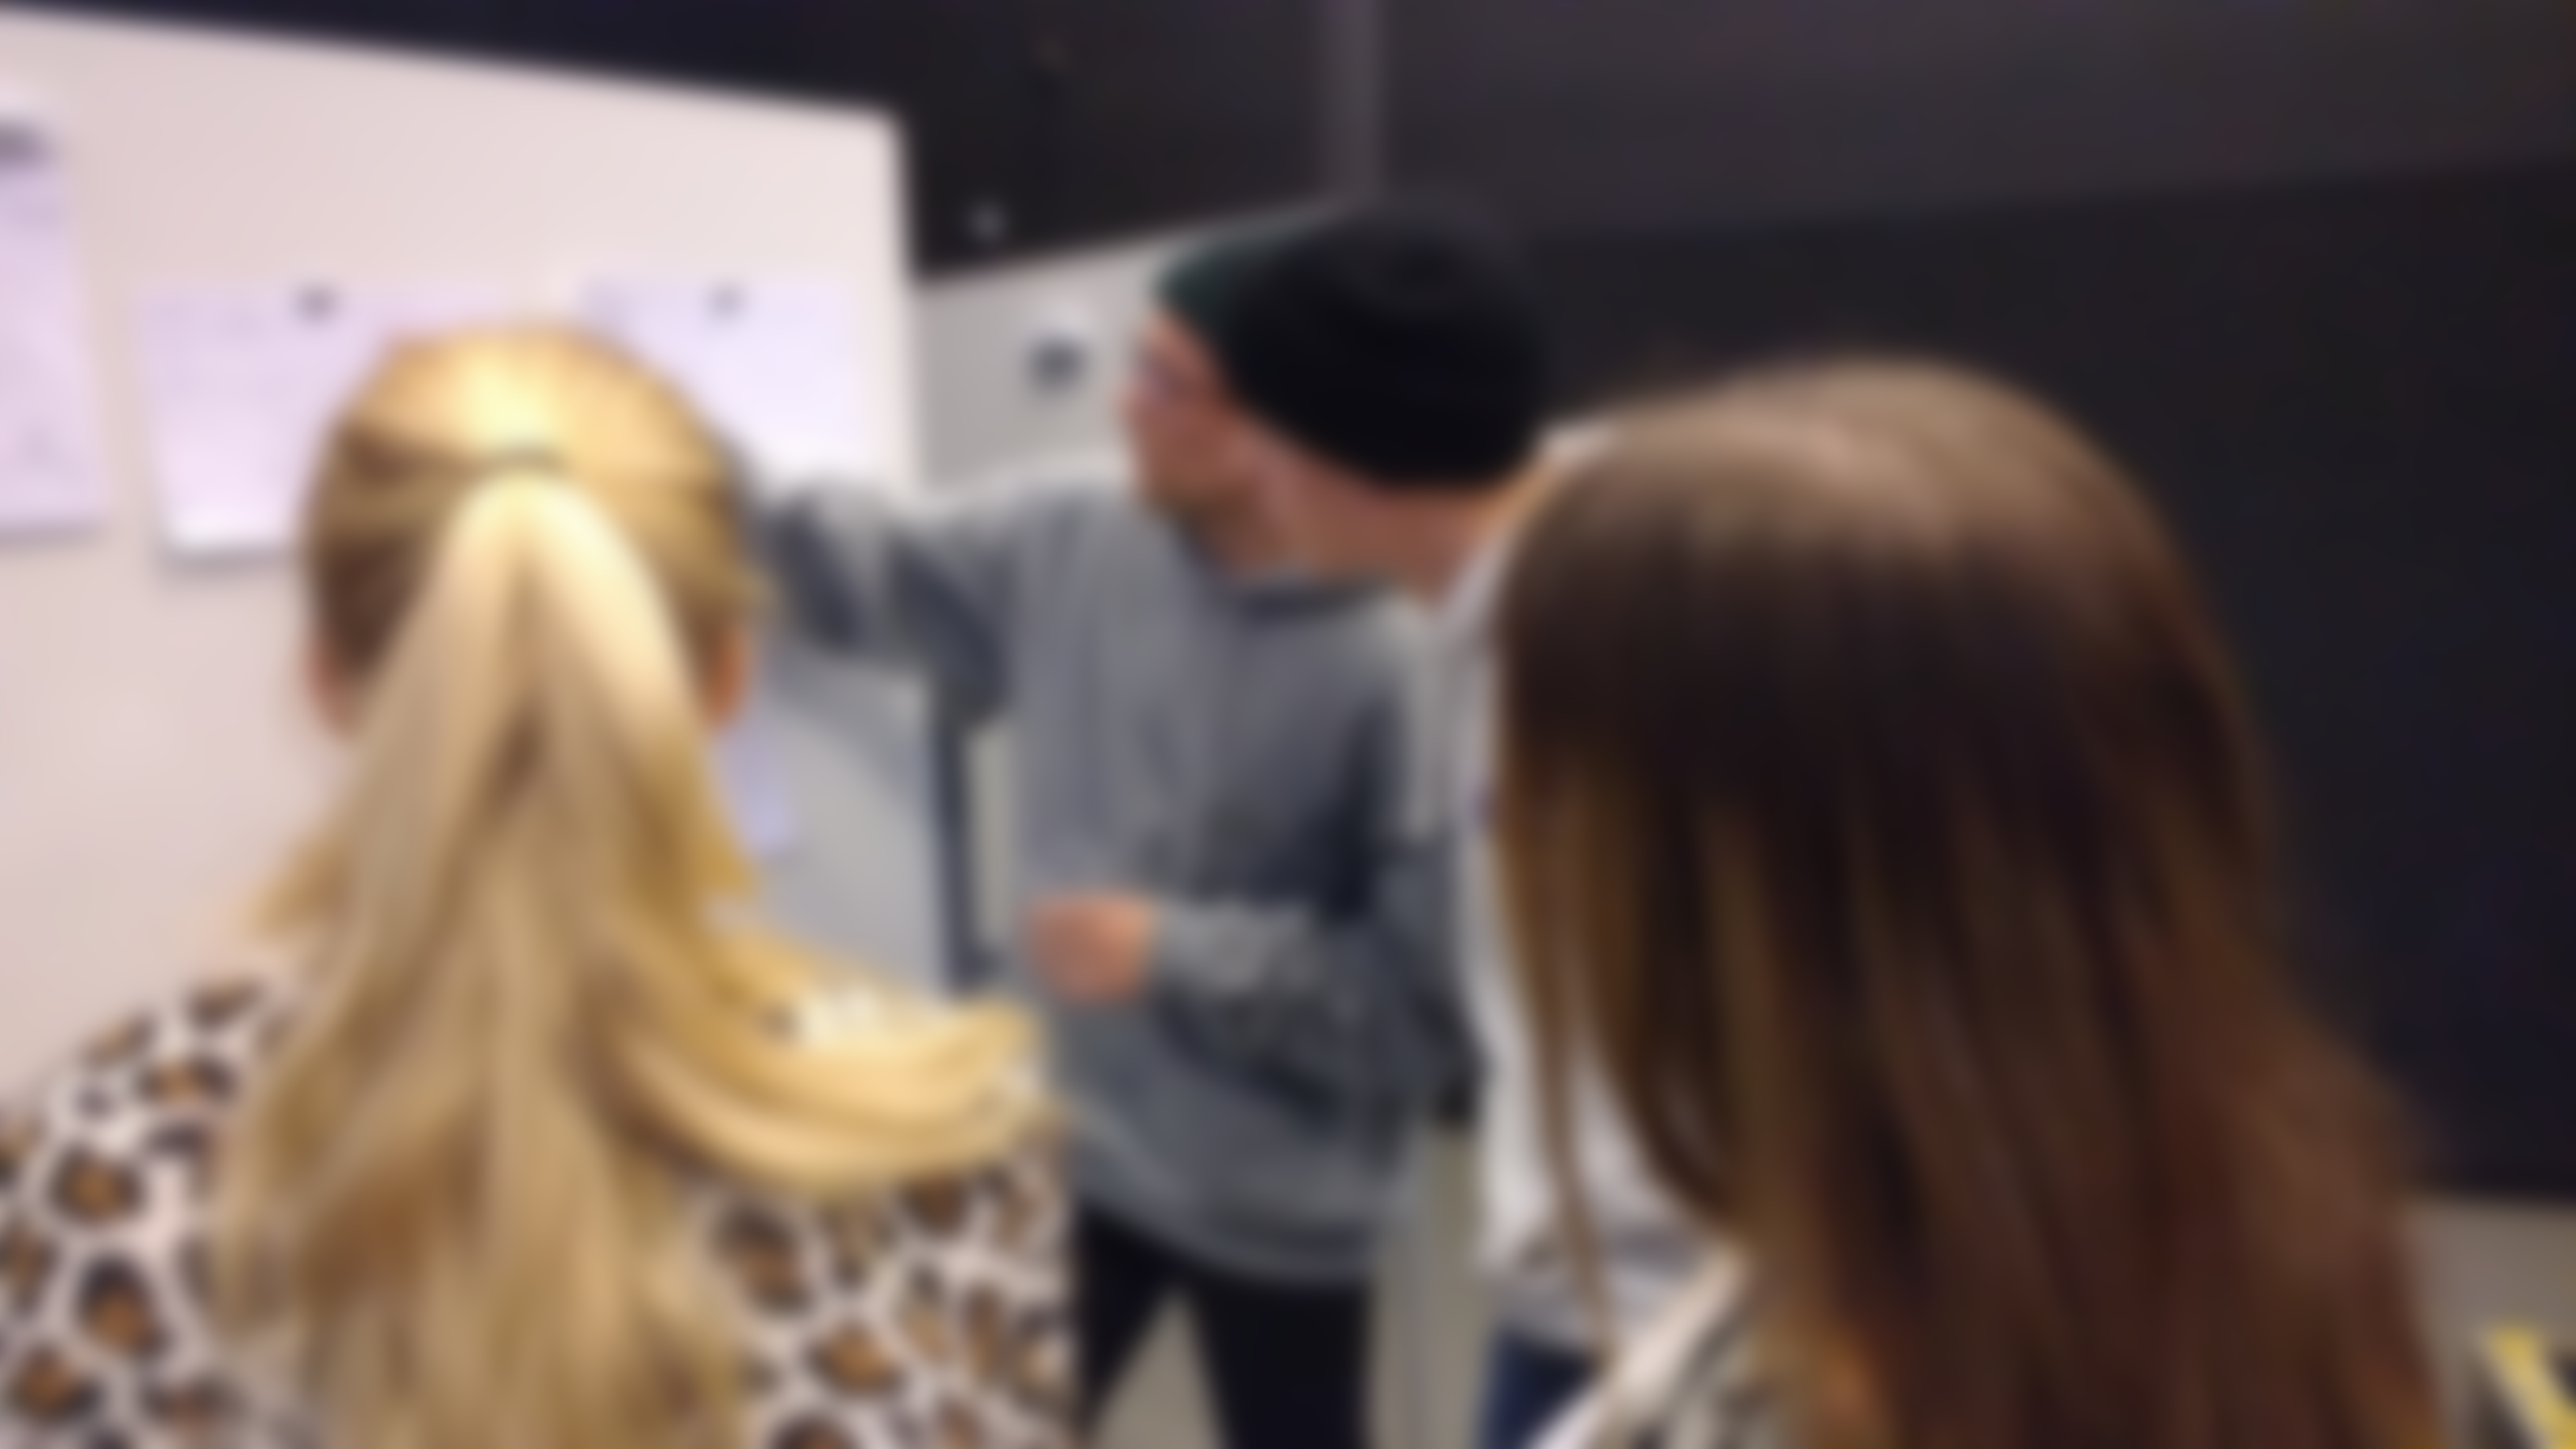
\includegraphics[width=24cm,height=13cm]{graphics/brainstormblur.png}
  }%
}
\begin{document}

\begin{titlepage}
\BgThispage
  %\vspace{12cm}
	\raggedright
  {\Large{\colorbox{front}{\color{white} \textbf{PROJECT NAME}\kern 1pc}}\\\vspace{0.3cm}}
  {Pilot Study\\}
  \vfill
	{\large \today\par}
  {\small\color{gray} Marc Coquand, Linus Lagerhjelm, Mattias Cederberg and Simon
  Asp\\}
  {\small\color{gray} Supervised by Stig Byström}\\
  {\small\color{gray} Umeå University\\}

	%\vfill

\end{titlepage}

\clearpage

\newpage
\backgroundsetup{
scale=1,
color=white,
opacity=1,
angle=0,
contents={%
  }%
}
\BgThispage

\pagecolor{front}\afterpage{\nopagecolor}\thispagestyle{empty}

\marginpar{\textcolor{white}{\small{Project
Management}\vspace{11cm}\\\large\textbf{Background}\\ {\small 
Walking home late at night can be a daunting experience. The newspapers write
about assaults and harassment, the northern winter climate contribute with
shorter days and darker nights. Existing street lights helps with the problem
but the feeling of uncertainty and fear persist. $PROJECTNAME$ will investigate
how a technical solution could be applied to create an increased sense of
safety. The project is carried out in collaboration with the municipality of
Umeå and Umeå University as part of the courses Interactivity in Smart
Environments and Project Management.
 }}} \newpage

\tableofcontents
\thispagestyle{empty}
\newpage

\section{Background}

\circuitfig{
\draw[white] (0,0)
to[R=$R_1$,color=white] (2,0) % The resistor
to[short] (2,2)
to[R=$R_1$,color=white] (2,0) % The resistor
to[short] (2,2)
to[V,v=$U_q$,color=white] (0,2) % The voltage source
to[short] (0,0);
}


\begin{leftsiderules}
Walking home late at night can be a daunting experience. The newspapers write
about assaults and harassment, the northern winter climate contribute with
shorter days and darker nights. Existing street lights helps with the problem
but the feeling of uncertainty and fear persist. $PROJECTNAME$ will investigate
how a technical solution could be applied to create an increased sense of
safety. The project is carried out in collaboration with the municipality of
Umeå and Umeå University as part of the courses Interactivity in Smart
Environments and Project Management
\end{leftsiderules}

\marginfig{graphics/brainstorm.jpg}{Our first brainstorming session}
\newpage

%\lipsum[4]

\begin{SCfigure}[][h]
  \caption*{\raggedleft {\small \textcolor{gray}{Installation, align this
  properly afterwards}}}
  \begin{minipage}[h]{\textwidth}
    \begin{lstlisting}
#include <stdio.h>
#define N 10
/* Block
 * comment */
    return 0;\end{lstlisting}
  \end{minipage}
\end{SCfigure}

\begin{SCfigure}[][h]
  \caption*{\raggedleft {\small \textcolor{gray}{continuation}}}
  \begin{minipage}[h]{\textwidth}
    \begin{lstlisting}
int main()
{
    int i;
    // Line comment.
    puts("Hello world!");
    for (i = 0; i < N; i++)
    {
        puts("LaTeX is also great for programmers!");
    }
    return 0;
}\end{lstlisting}
  \end{minipage}
\end{SCfigure}

\section {blank}
Walking home late at night can be a daunting experience. The newspapers write
about assaults and harassment, the northern winter climate contribute with
shorter days and darker nights. Existing street lights helps with the problem
but the feeling of uncertainty and fear persist. $PROJECTNAME$ will investigate
\marginquote{``This is a very inspirational quote right here. Very
quoteworthy if I may say so myself.''}
how a technical solution could be applied to create an increased sense of
safety. The project is carried out in collaboration with the municipality of
Umeå and Umeå University as part of the courses Interactivity in Smart
Environments and Project Management
\newpage
\end{document}
